%!TEX root = ../../main.tex

\section{Entity-based Event Detection Approach}
\label{detection:sec:approach}
In this section we describe our entity-based event detection approach.
The approach comprises of 6 key stages, as shown in Figure \ref{detection:graphic:pipeline}.
Tweets are processed in order using a pipelines architecture that allows for parallel processing, with each component relying only on the output of the previous component to complete its task.

\vspace{0.5cm}
\begin{figure}[h!]
	\centering
	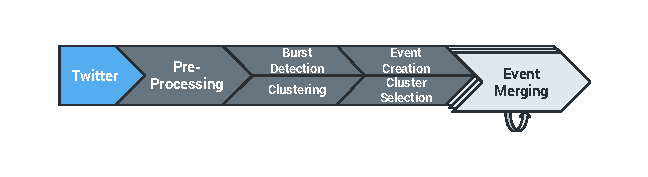
\includegraphics[width=11cm,trim=1.5cm 1cm 1.5cm 0.8cm]{Chapters/EntityDetection/images/system.pdf}
	\caption{The pipeline architecture and components of our entity-based approach.}
	\label{detection:graphic:pipeline}
\end{figure}

\subsection{Tweet Pre-processing}
Our approach uses a number of pre-processing steps.
This helps to filter out unwanted tweets, such as common types of spam, and attempts to provide a noise free stream of tweets which can used to detect events.

\subsubsection{Parsing \& Tagging}
\label{detection:sec:parsing}
We use the Stanford CoreNLP Natural Language Toolkit to perform Part of Speech (POS) tagging and Named Entity Recognition (NER) on the text of each tweet.
We  use the GATE Twitter POS model~\citep{TwitterPOS} for Part of Speech tagging, and the Stanford 3 class model for Named Entity Recognition.
The GATE Twitter POS model is a Part-of-speech models trained specifically on tweets and tends to provide much high accuracy ($>$ 90\%) that part-of-speech models trained on non-twitter corpora.

We extract all nouns, verbs and named entities from each tweet.
Nouns and verbs are lemmatized, and entities are kept in their longest form to ensure that names are as distinguishing as possible  (i.e. ``Paul Ryan'' rather than ``Paul'' and ``Ryan'').

The Stanford 3 class NER model is able to perform automatic class-based disambiguation such that entity mentions are also give a class (person, location, or organization).
We use this class information and consider named entities of different classes to be distinct, even if the name itself is identical.
For example, the entity ``Spain'' in the context of the football team (an \emph{organization} consisting on many people that play football) is conceptually different from ``Spain'' the (the landmass, a \emph{location}), as this helps to retain as much distinguishing power as possible.
We evaluate and give reasoning for this choice in section \ref{detection:sec:entityTypes}.
All terms and entities are converted to lowercase and any non-alphanumeric characters are removed (however whitespace is retained in the case of named entities).

\subsubsection{Filtering}
Event detection is analogous to a filtering task in many ways -- by removing as many non-event related tweets as possible, we are more likely to find event related ones. To this end, we apply a set of filters which remove over 95\% of tweets.
This has a number of benefits.
Firstly, assuming that the filters remove more noise than signal, it becomes considerably easier to extract events.
Secondly, unlike other approaches which filter after clustering~\citep{Petrovic:2010:SFS:1857999.1858020,becker2011beyond}, filtering before clustering reduces the amount of data which needs to be processed, and plays a significant role in the ability of our approach to detect events in a time and space efficient manner.

We first remove tweets that contain no named entities.
This is our most aggressive filter, removing over 90\% of tweets.
As discussed in section \ref{detection:sec:entityEvents}, we believe that named entities play a crucial role in describing events, thus do not believe that this filter significantly harms detection performance, and provide some evidence towards this in section \ref{detection:sec:entitiesEval}.
Furthermore, in order to efficiently cluster tweets, our clustering approach (described in section~\ref{detection:sec:clustering}) requires each tweet to contain at least one named entity, making this filter necessary.

We also remove retweets, which make up approximately 30\% of all tweets and are simply a copy of an existing tweet.
Retweets require little effort to produce, meaning that they are often associated with the spread of spam, memes and misinformation~\citep{Grier:2010:SUC:1866307.1866311}, and do not provide any new information.
We examine the effect of removing retweets in section \ref{detection:sec:retweetsEval}, and show that their removal improves precision.

We also use a range of term-level filters that remove terms and entities that are unlikely to be related to an event or that are known to be associated with spam and noise.
As well as stop words and expletives, we remove terms associated with watching television (``watch'', ``film'',``movie'', ``episode'', etc.) or listening to music (``listen'', ``song'', ``play'', etc.).
This helps to reduce the number of false positives created by large numbers of users watching a television show while using a ``second screen'' to discuss it, as significant, but fictional events in television shows can often cause reactions that appear similar to real-world events.
We also remove terms and entities associated with traditional news and broadcast agencies, such as ``bbc news'', ``cnn'', ``fox news'' and ``reuters''.
Tweets from these agencies often contain their own name, which can cause issues with our entity based clustering and merging approaches (described in sections \ref{detection:sec:clustering} and \ref{detection:sec:entityLinking}) as the same entity can appear to be associated with a large number of events simultaneously.
Term level filters such as these are likely to require some maintenance as the usage of Twitter continues to evolve and require some domain knowledge to construct, however this small amount of expert work helps to remove vast amounts of noise.
Finally, terms under 3 characters in length are removed.

\subsection{Entity-based Online Clustering}
\label{detection:sec:clustering}
Nearest-neighbor clustering is a commonly used method in event detection to find documents that discuss a similar topic or event, however it is also inherently slow when dealing with large numbers of documents, making traditional clustering approaches, such as those used by the TDT project described in section \ref{background:alg:tdt}, infeasible at Twitter scale.
A number of solutions have been proposed to solve this, including the use of Locality Sensitive Hashing~\citep{Petrovic10}, which we implement in chapter \ref{chapter:collection}.
However, these approaches are general purpose, and do not make use of any domain or task specific information.
Given the role that named entities play in describing real-world events, we believe it makes sense to use their presence to improve clustering efficiency and effectiveness for the task of event detection.

Using the premise that tweets discussing an event must contain at least one of the named entities involved in the event, we partition tweets based upon the entities they contain, and add a tweet to a cluster for every entity it contains, as show in in Figure \ref{detection:graphic:clustering}.

\begin{figure}[h!]
	\centering
	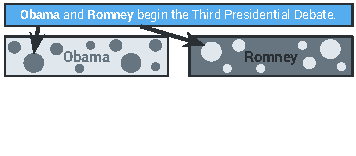
\includegraphics[width=8cm,trim=0cm 1.5cm 0cm 0cm]{Chapters/EntityDetection/images/clustering.pdf}
	\caption[Entity-based clustering]{Tweets are added to a cluster for each entity they contain. The example shows how a tweet containing both `Obama' and `Romney' would be put into two clusters, one for the entity `Obama' and one for the entity `Romney'.}
	\label{detection:graphic:clustering}
\end{figure}

For the purpose of clustering, this can be thought of as having a unique inverted index for every named entity. For each named entity $e$ in tweet $d$, a list of tweets $D$ is retrieved from the inverted index for $e$ (the inverted index for $e$ does not contain a row for $e$) and the maximum TF-IDF weight cosine similarity score is calculated between $d$ and each tweet in $D$.

To ensure that our approach is able to run in real-time, we limit the number of tweets that can be retrieved from an entity's inverted index to a fixed number per term (usually between 100-1000), and use only the top 10 TF-IDF weighed terms per tweet. Less than 1\% of tweets from our test collection contain more than 10 terms, meaning that we lose very little information by enforcing this limit, whilst ensuring an upper bound of \(10N\) comparisons are made, where \(N\) is the maximum number of documents retrieved per term. Nouns, verbs and named entities are used when calculating the cosine similarity between tweets, however the named entity whose inverted index was used to retrieve comparison documents is given a weight of 0 in order to give as much weight as possible to other topical terms.

If the maximum score is above a set threshold (usually in the range \(0.4-0.6\) \citep{Petrovic10}, discussed in section \ref{detection:sec:simThresholds}), then $d$ is added to the same cluster as its nearest neighbour. If the nearest neighbour does not already belong to a cluster, then a new cluster is created containing both tweets and assigned to entity $e$. The new tweet is then added to the inverted index for entity $e$.

It should be noted that unlike traditional event detection approaches, we do not assume that the formation of a new cluster indicates a new event. Algorithm \ref{detection:alg:clustering} shows the pseudocode for our entity based cluster approach.

\begin{algorithm}
	\DontPrintSemicolon
	\KwIn{Minimum similarity threshold $m$}
	index $\gets [][]$ \\
	clusters $\gets$ [][] \\

\ForEach{tweet d in the stream} {

	\ForEach{entity e in d} {

		$S(d) \gets \emptyset$ \tcp*{set of documents that share a term with $d$}
		\ForEach{non-entity term t in d} {
			\ForEach{tweet d' in index[e][t]} {
				$S(d) \gets S(d) \cup d'$ \\
			}
			index[$e$][$t$] $\gets$ index[$e$][$t$] $\cup$ $d$ \\
		}

		$c_{max} \gets 0$ \tcp*{maximum cosine between $d$ and tweets in $S(d)$}
		$n_{d} \gets nil$ \tcp*{tweet with maximum cosine to $d$}
		\ForEach{tweet d' in S(d)}{
			$c$ := cosine($d$, $d'$) \\
			\If{$c > c_{max}$}{
				$c_{max} \gets c$ \\
				$n_d \gets d'$
			}
		}

		\eIf{$c_{max} \geq m$} {
			add $d$ to clusters[$e$][$n_d$]
		}{
			clusters[$e$][$d$] $\gets$ new cluster($d$) \tcp*{Do not assume the cluster is a new event}
		}

	}
}

\caption{Entity-based method of clustering}
\label{detection:alg:clustering}
\end{algorithm}

\subsection{Identifying Bursty Entities}
For an effective event detection approach, it is important to have a method of detecting significant events and filtering the mundane. We do this by looking for temporal bursts in the frequency of an entity, which can occur over periods ranging from a few minutes to several hours. To model this, we use a set of windows for each entity to capture their frequency over time, starting at a 5 minutes, and doubling in length up to 320 minutes (i.e. 5, 10, 20, \ldots, 320).

We use the Three Sigma Rule as the basis for a light-weight burst detection approach, which states that a value is considered to be practically impossible if it is further than 3 standard deviations from the expected value \citep{Pukelsheim94}. For the windows, we maintain mean and standard deviation values, updating them periodically with the current entity frequency. It is possible to efficiently compute moving mean (\(\mu\)) and standard deviation (\(\sigma\)) values using a set of three power sums \(s_0\), \(s_1\) and \(s_2\), where \(s_j\), \(\mu\) and \(\sigma\) at time period \(n+1\) for data series \(x\) is shown below:
\[
s_{jn+1}= s_{jn} + x_{n+1}^j
\]
The current mean and standard deviation values (\(\mu\) and \(\sigma\) respectively), can then calculated as so:
\begin{equation*}
	\begin{aligned}[c]
		\mu = \frac{s_1}{s_0}
	\end{aligned}
	\qquad\qquad
	\begin{aligned}[c]
		\sigma = \sqrt{\frac{s_0 s_2 - s_1^2}{s_0}}
	\end{aligned}
\end{equation*}

The \(\mu\) and \(\sigma\) values for each window are updated periodically based upon the length of the window (i.e., a 5 minute window is updated every 5 minutes).
In our evaluations, we find that using full historic frequency information for each window (section \ref{detection:sec:burstDetection}), and instead use only the past 12 values to calculate mean and standard deviations.

When a tweet which is no longer covered by the largest window it is removed from all inverted indexes. This helps to reduce the number of comparisons required when calculating the nearest neighbour, and allows resources to be freed for incoming tweets. We do not believe that removing older tweets will affect the effectiveness of the algorithm due to the real-time nature of Twitter, as tweets which are more than a few hours old are generally not relevant to any ongoing real-world events, and those which are will hopefully have already been marked as so by the algorithm, ensuring that they are recorded elsewhere.

Once a tweet has been clustered and added to entity indexes (as shown in Algorithm \ref{detection:alg:clustering}), we update the entity statistics, and check if the newly added tweet caused the entity to burst in any of the windows. If the number of tweets in a given window is greater than \(\mu + (3 \cdot \sigma)\), then we say that the given window is bursty, and the entity is part of a new event.

In order to smooth and reduce noise, statistics are not updated while a window is bursting, and windows are kept in a bursting state for \(1.5 \times window\_length\) after the window's statistics suggest that it has stopped bursting. For example, an entity which is marked as bursty in the 80 minute window would remain bursting for 120 minutes after the 80 minute window stops bursting.  The extra time allows for fluctuations in frequency as an event develops, and helps prevent a state of flux where an entity rapidly switches between bursting and normal states.

\subsection{Event Creation and Cluster Selection}
\label{detection:sec:eventCreation}
Once a burst has been detected, an event is created and associated with the bursting entity for the duration of the burst (we address how an event could be associated with multiple entities in section \ref{detection:sec:entityLinking}).
However, the event does not yet have any tweets associated with it.
We cannot simply take all of the tweets posted during the burst as these will contain background topics about an entity, such as discussion about visiting a location or listening to a particular artist's music. To solve this, we propose the use of a number of heuristics to select significant clusters which are the most likely to be related to the event that caused the burst.

We require that the centroid time of a cluster (i.e. the average timestamp associated with all tweets in a cluster) is greater than \(B_e\), where \(B_e\) is the time at which the entity began to burst. This helps to ensure that clusters which discuss background topics are not included as they are likely to have existed for some time before the burst took place. A cluster's centroid time is updated as new tweets are added, ensuring that clusters which initially had a centroid time prior to the burst can still be added to an event. This is important as it allows clusters containing early reports of the event, which often occur before any burst takes places, to be included.

We also require that a cluster meets a minimum size threshold, usually between 5 and 20 tweets (10 is used for our evaluations).
This is to ensure that the cluster covers a significant portion of the event and to prevent small but noisy clusters from being included. The minimum size has an effect on the precision of our approach, and large minimum cluster sizes can give a large increase in precision for a small reduction in recall. We discuss the minimum cluster size in detail in section \ref{detection:sec:simThresholds}.

An event is kept alive as long as it has at least one bursting entity associated with it. Once all entities associated with an event have stopped bursting, the event is finalized, and no more clusters or tweets can be added to it.

\subsection{Event Merging and Entity Linking}
\label{detection:sec:entityLinking}
New events are related to only a single entity.
However, most events involve more than one entity, such as a person and a location, or an interaction between two organizations.
In additional, events are often discussed using a number of synonyms.
For example ``Barack Obama'' is often shorted to simply ``Obama''.
These issues mean that there are generally a number of Event objects, each created by separate named entities but of which discuss the same real-world event.
To solve this, we create links between events which are related to the same real-world event using entity co-occurrence statistics.
If an entity is mentioned in at least 50\% of tweets in an event, then we say there is a potential link between the event and the entity.

If such a potential link is found, a number of checks are performed to ensure that the entity is viable and likely to be related to the event. Firstly, we check that the potential entity is bursting and therefore is already associated with an event. Secondly, we verify that the entity has not already been associated with the event. This requirement prevents long-running events from consuming popular or frequently bursting entities. For example, an event which is associated with both ``Obama'' and ``Romney'' would not automatically be merged with `Romney' should it stop bursting and then burst again before the original event had finished. Instead, the Romney entity would form a new event, which may then link itself to the previous event if Obama occurs in more than 50\% of tweets.

If event $E_{1}$ finds a potential link with entity $e$, and entity $e$ passes both of the above checks, then event $E_1$ is merged with the event belonging to $e$. This merging process can happen any number of times to produce events with many entities, and consisting of all the clusters and tweets from both.
Entity frequencies are then recalculated and any new semantic links are then followed to merge yet more events.

Once an entity has stopped bursting, it is no longer linked with an Event and no new clusters from that entity are added.
However, clusters for an entity which have already been added are still updated, and any new tweets are reflected in the entity frequencies for the event.
Events are kept active until they contain no more active entities and all clusters in the event have become inactive (i.e. all the of the tweets in the cluster have been removed from the inverted index associated with its entity).
This helps to capture more information about the event, even after discussion has died down.

\subsubsection{Entity Normalization}
\label{sec:entityNorm}
As described in section \ref{detection:sec:clustering}, entities are kept in their longest form rather than split into individual components (e.g. `Barack Obama', rather than `Barack' and `Obama').
However, this can cause issues as multiple events are created for different forms of the same entity.
Using our previous example, it is unlikely that single tweet will mention both `Barck Obama' and `Obama', resulting in two separate events that our entity linking approach is unlikely to merge.

To solve this, we perform a naive entity normalization technique.
When measuring the frequency of entity mentions within an event, we perform a normalization step, which counts the last term of people and organization names as a separate entity.
For example, for event mention of `barack obama', we also increase the count of `obama'.
Note that we only do this for People and Organizations, but not Locations, as locations tend to lose much of their meaning when split (e.g. United Kingdom $\rightarrow$ Kingdom).